\documentclass[12pt] {article}
\usepackage{times}
\usepackage[margin=0.8in,bottom=1in,top=0.7in]{geometry}

\usepackage{hhline}
\usepackage{subfig}
\usepackage{graphicx}
\begin{document}

\title{Performance Characterization -  EEC289Q}
\author{Ahmed H. Mahmoud}
\date{January 25th, 2018}
\maketitle
%============Table========
%\begin{figure}[tbh]
% \centering    
%\begin{tabular}{ |p{4cm}|| p{2cm}|p{2cm}|p{2cm}|p{2cm}|}
% \hline
% & Processor 1 &  Processor 2  & Processor 3 & Processor 4\\ \hhline{|=|=|=|=|=|}
% \hline
% Performance          &$1.08$        &$1.425$       &\textbf{1.52}  &   \\
% \hline
%\end{tabular} 
%\caption{Metric table for the four processors}
%   \label{tab:metric}
%\end{figure} 
%============Figure========
%\begin{figure}[!tbh]
%\centering        
%   \subfloat {\includegraphics[width=0.65\textwidth]{fig2_4.png}}
%   \caption{ }
%   \label{fig:fig}
%\end{figure}

%============Part One========
\paragraph{Part One:}
Figure~\ref{fig:part1} shows the experiments with different number of threads and blocks on both devices. For fixed number of blocks, we notice that the maximum BW achieved always coincides with number of threads being multiple of the warp size (32). This is particularly visible on the K40 device. This is because all the threads within a warp would be doing some useful that contribute to the final results.On this graph, the maximum achieved BW is \emph{probably} limited by the number of blocks since the same number of blocks were used on the K620 device and the maximum achieved BW reached up to 90\% of the hardware limit. Also, with fewer threads per block, one thread will be doing more work which increases the run time and decreased the achieved BW (left side of the plot). On the K620, the achieved BW leveled off when the number of threads meets limit on the number of warps resident on SM. For compute capability (source Wikipedia), the maximum number of resident blocks per SM is 32 which is always satisfied for out configuration. The max resident warps is 64 and max resident threads is 2048. Thus, since we already have more than 32 blocks at a time, the maximum utilization we can achieve is when the number of threads is 64 ($2048/32=64$) which is the point at which the curve level off. Same analysis goes for fixing the number of threads while varying number of blocks in which the curve flattens with 8 blocks on K620 device; the 256 threads give 8 warps and would need 8 blocks to get to 32 warps resident. 

\begin{figure}[!tbh]
\centering        
   \subfloat {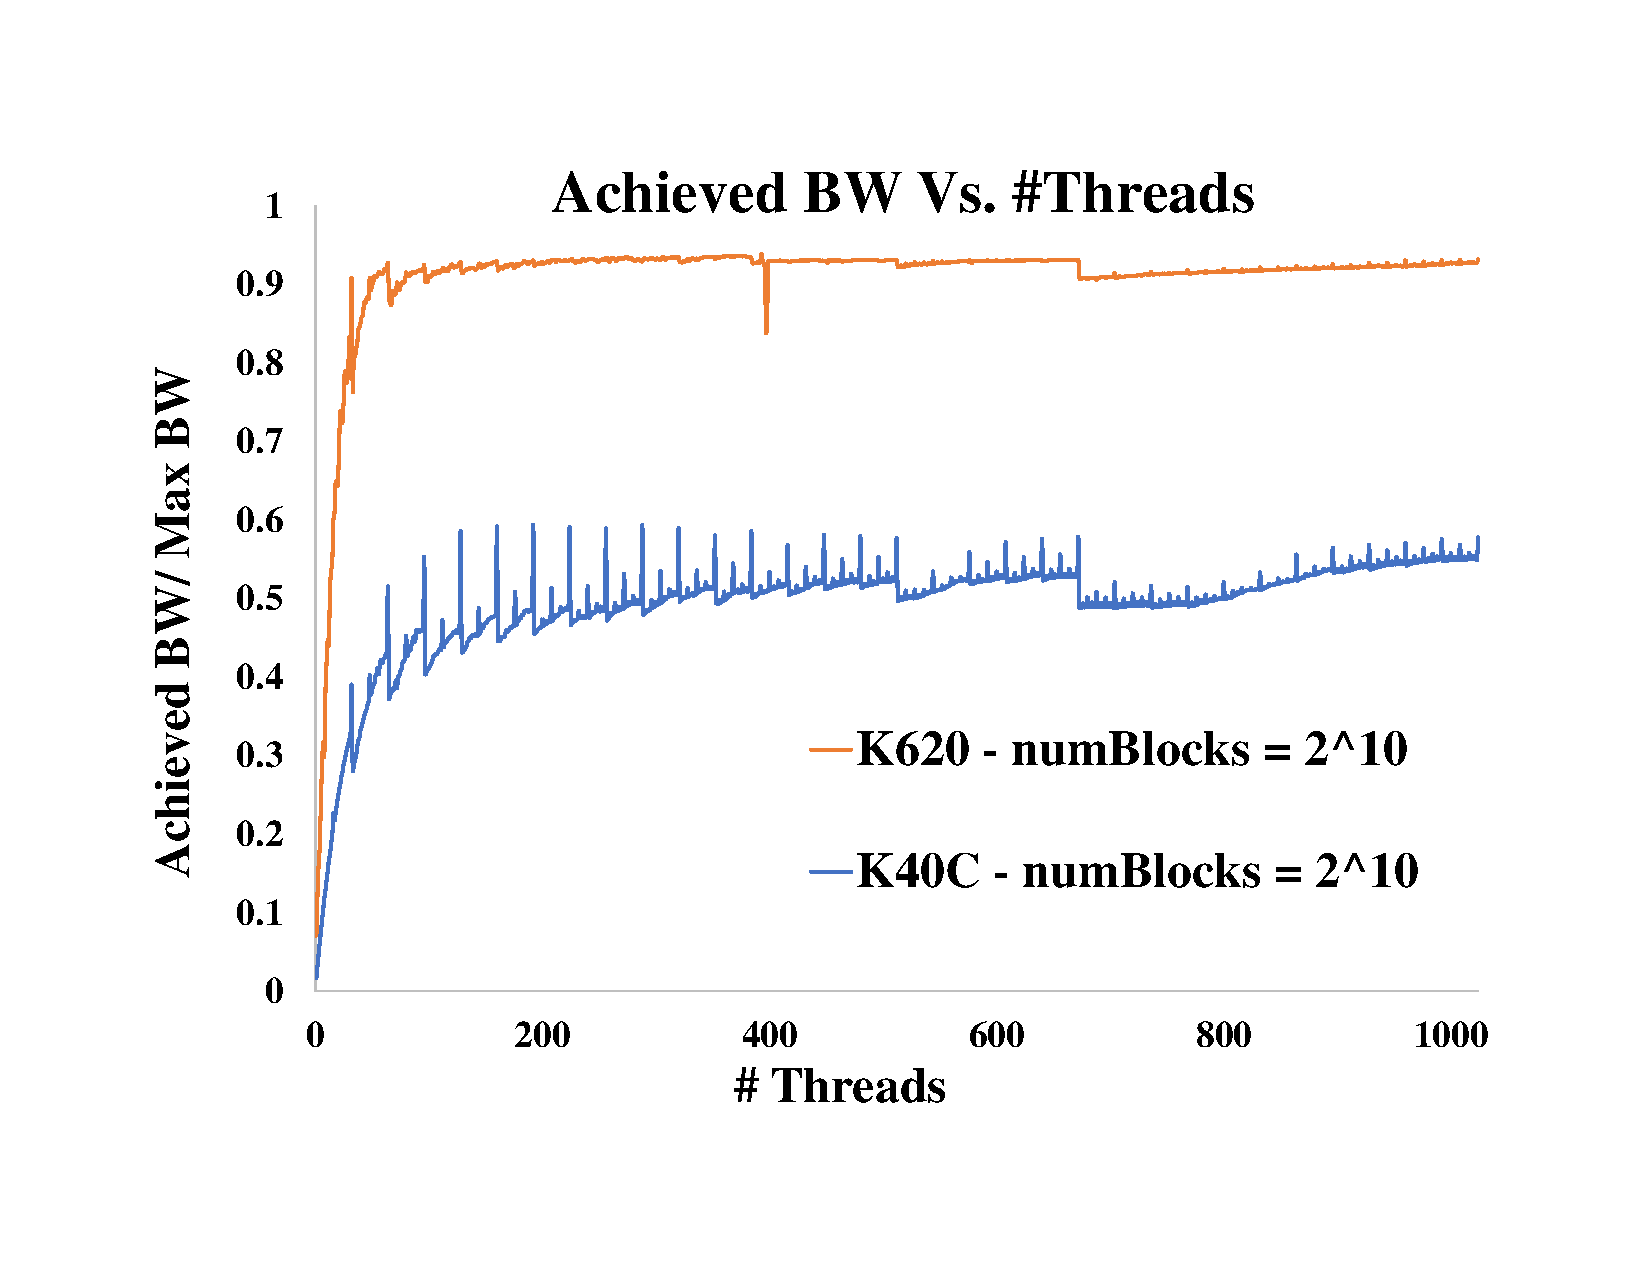
\includegraphics[width=0.49\textwidth]{fig/thds.pdf}}
   \subfloat {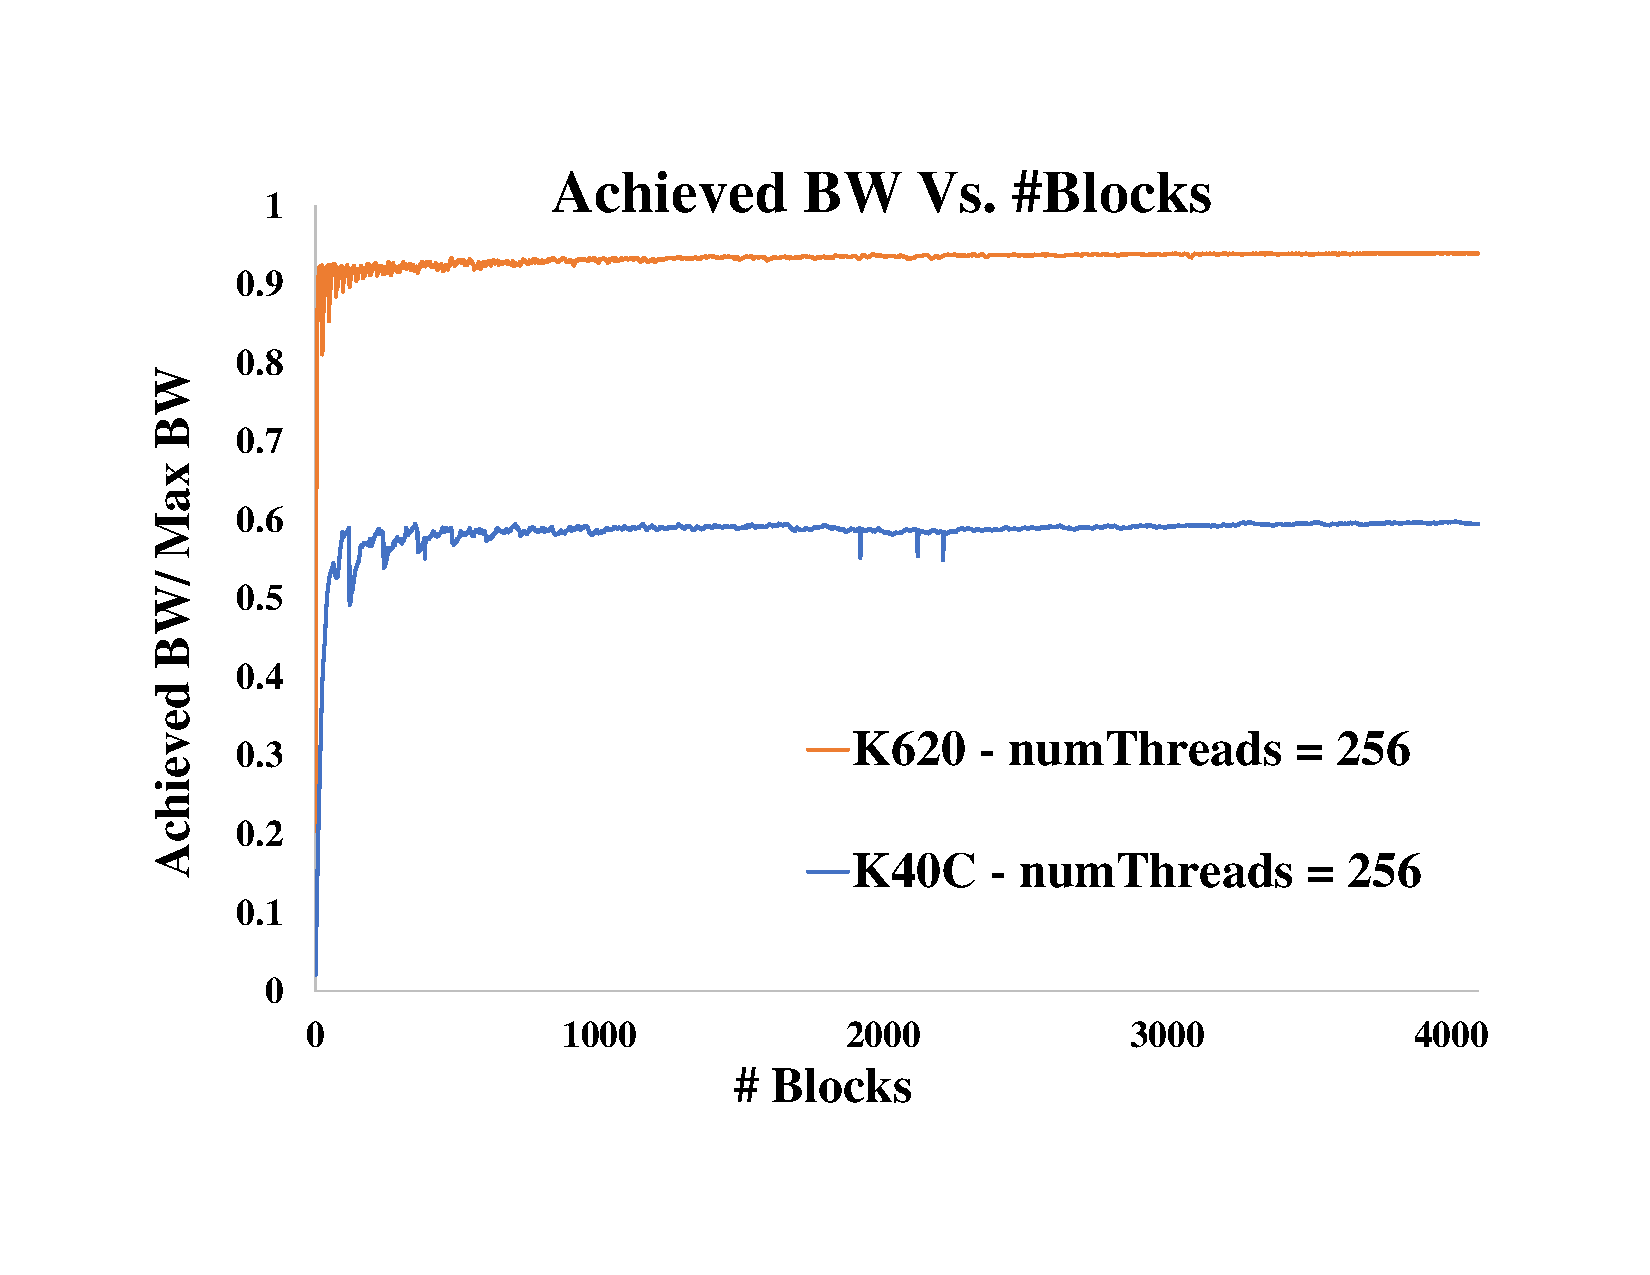
\includegraphics[width=0.49\textwidth]{fig/blcks.pdf}}
    
   \caption{Experimenting with different number of threads (while fixing number of blocks) and different number of blocks (while fixing number of threads) on both Kepler K40 and Quadro K620 devices. Array of length is $2^{20}$.}
   \label{fig:part1}
\end{figure}


 

%============Part Two========
\paragraph{Part Two:}
Here we answer the questions on \textbf{bold} as shown in the assignment. Here, we always used array on length $2^{20}$ on the K620 device. 

\begin{enumerate}
\item  Using 4320 blocks and 64 threads on K40 device, the achieved BW was $55.4\%$ of the maximum BW. The total number of memory operations is $2(reads)*1(write)*N(array\_len)$. The running time was $0.0747\ mSec$. We were able to increase this number to be just $58.3\%$ by using \texttt{float4} instead of \texttt{float}, adjusting the number of threads and blocks to be 64 threads and 4096 blocks and use loop unrolling and preferring more L1 cache using \texttt{cudaFuncCachePreferL1}. This code took $0.07105\ mSec$. 

\item The FLOPS ($13.6933\ GFLOPS$) of this code is $0.3191\%$ of the maximum achievable. The total number of floating point operations is the length of the array. We were able to increase the achieved GFLOPS to be $88.7\%$ of the maximum achievable ($3806.77\ GFLOPS$) by 1) doing multiply-add instead of just add, 2) reading the value into registers and do $600$ multiply-add on the two values being read by each threads using (unrolled) loop and then write to global memory, and  3) using larger few blocks i.e., 1024 blocks with 256 threads. The run time of this code is 0.4617 mSec, 


\item The arithmetic intensity from Part 2.1 is $1176.43\ FLOPs/Byte$ and from Part 2.2 is\\ $324740\ FLOPs/Byte$.

\item For this part we fixed the number of memory operations to be similar to other parts i.e., $2(reads)*1(write)*N(array_len)$. We changing the number of operations by varying the 600 number from part 2.2 to start from 1 up to 600. Figure~\ref{fig:part2} shows the achieved arithmetic intensity. We can see that the balance point occurs at around $240906\ FLOPs/Byte$ at which $65.788\%$ of the maximum FLOPS was achieved ($2823.12\ GFLOPS$).
\begin{figure}[!tbh]
\centering        
   \subfloat {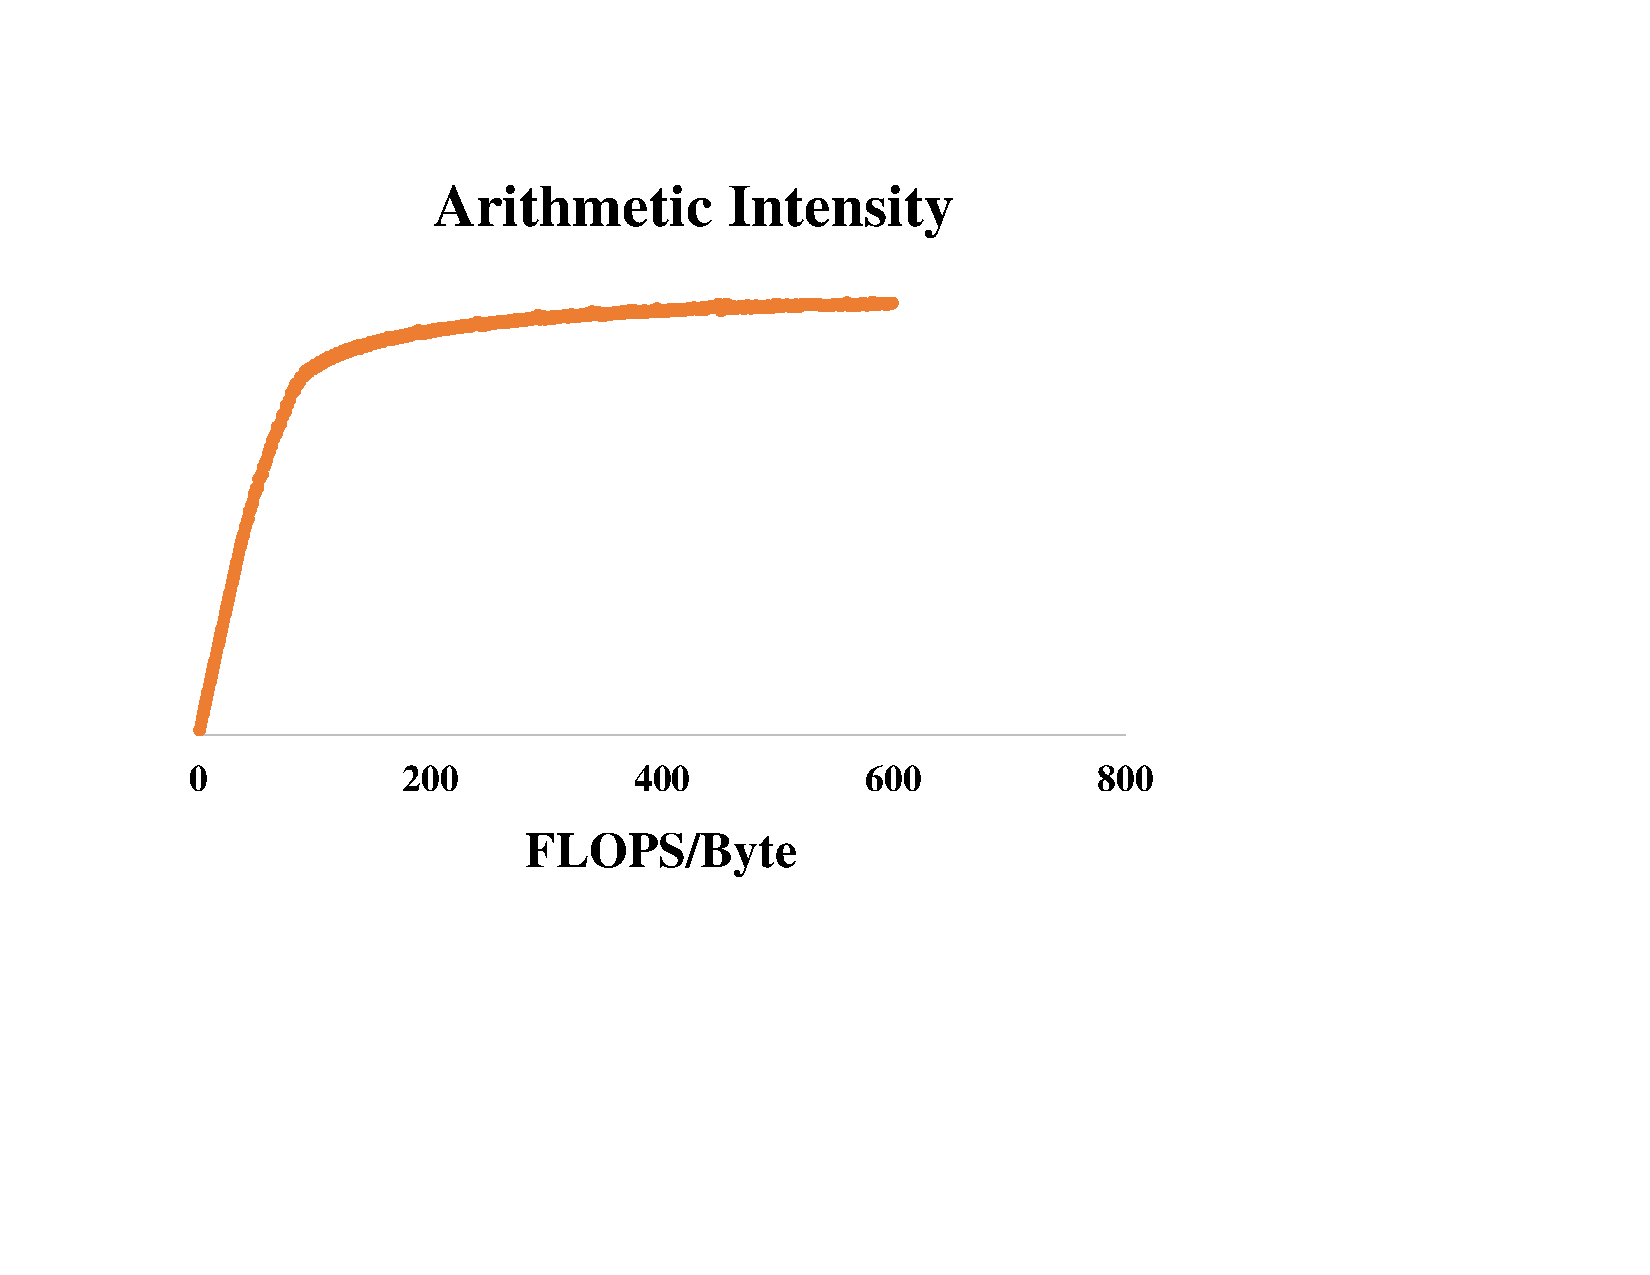
\includegraphics[width=0.7\textwidth]{fig/arth.pdf}}
   \caption{Recording of the arithmetic intensity while increasing the number of operations.}
   \label{fig:part2}
\end{figure}


\end{enumerate}




\end{document}
